% !TEX TS-program = pdflatex
% !TEX encoding = UTF-8 Unicode

%%% PAGE DIMENSIONS 16:9
\documentclass[11pt, notheorems, aspectratio=169]{beamer}

%%% TEXT FEATURES
\usepackage[utf8]{inputenc} % set input encoding (not needed with XeLaTeX)
\usepackage[T2A]{fontenc} % font encoding
\usepackage[russian]{babel} % languages
\usepackage{amsfonts} % for natural, rational, etc numbers
\usepackage{amsmath} % special math symbols
\usepackage{amssymb} % some more special symbols
\usepackage{color, colortbl}
\setbeamertemplate{navigation symbols}{}
\renewcommand{\arraystretch}{1.5}
\usefonttheme{serif}

%%% COLORIZING FEATURES

% color theme settings
\mode<presentation>
{
  \usetheme{AnnArbor}
  \usecolortheme{beaver}
  %\setbeamercovered{transparent}
}
\setbeamercolor{frametitle}{use=structure, bg=gray-background, fg=dark}
\setbeamercolor{palette primary}{bg=dark, fg=white}
\setbeamercolor{palette secondary}{bg=light, fg=white}
\setbeamercolor{palette tertiary}{bg=medium, fg=white}

% frame title settings
\setbeamertemplate{frametitle}
{
    \nointerlineskip
    \begin{beamercolorbox}[sep=0.3cm,ht=1.8em,wd=\paperwidth]{frametitle}
        \strut\textbf{\insertframetitle}\strut
        \vskip-1ex%
    \end{beamercolorbox}
}

\graphicspath{{../images/}}
\setbeamerfont{footnote}{size=\tiny}

% colored theorem blocks
%\setbeamercolor{block title}{use=structure,fg=white,bg=medium}
%\setbeamercolor{block body}{use=structure,bg=light!10}

% colored tables
\usepackage{colortbl}
\usepackage{tabularray}

% colored captions
\usepackage{caption}
\DeclareCaptionLabelFormat{mycaption}{\usebeamercolor[medium]{caption name} #1 #2: }
\captionsetup[figure]{labelformat=mycaption, labelsep=none, labelfont=bf}
\captionsetup[table]{labelformat=mycaption, labelsep=none, labelfont=bf}

% colored lists (light-blue squares)
\usepackage{enumitem, xcolor}
\newlist{coloritemize}{itemize}{1}
\setlist[coloritemize]{label=\textcolor{light}{$\blacksquare$}}
\colorlet{itemizecolor}{.}% Default colour for \item in itemizecolor
%%%%%%%%%%%%%%%%%%%%%%%%%%%%%%%%%%%%%%%%%%%%%%%%%%%%%%%%%%%%%%%%%%%%%%%%%%%%%%%
%%% To use a different custom template in the {coloritemize} environment,   %%%
%%% set item parameters:                                                    %%%
%%%                                                                         %%%
%%% \begin{coloritemize}                                                    %%%
%%%     \item[{$\color{medium}\blacksquare$}]                               %%%
%%% \end{coloritemize}                                                      %%%
%%%%%%%%%%%%%%%%%%%%%%%%%%%%%%%%%%%%%%%%%%%%%%%%%%%%%%%%%%%%%%%%%%%%%%%%%%%%%%%
\definecolor{Gray}{gray}{0.9}
% bordered text
\usepackage[most]{tcolorbox}
\newtcolorbox{myblock}[1][]{
    enhanced jigsaw,
    colback=gray-background,
    colbacktitle=gray-background,
    coltitle=black,
    %colframe=blue!85!white!90!,%
    %size=small,%
    %boxrule=1pt,%
    halign title=flush left,%
    %coltitle=blue,%
    breakable,%
    drop fuzzy shadow=black!70!white,%
    left=0pt,
    titlerule=0pt,
    top=1pt,
    bottom=0pt,
    enlarge left by=-0.1cm,
    grow to right by=0.21cm,
    frame empty,
    borderline={0.3mm}{0mm}{dark},
    title={\textbf{#1}}
}

%\newcommand{\mycitation}[2]{\myblock{\textbf{#1}}{#2}}

\newtcolorbox{mybox}[1][]{
    colback=white,
    colbacktitle=white,
    coltitle=red!70!black,
    colframe=red!70!black,
    boxrule=1pt,
    titlerule=0pt,
    arc=15pt,
    title={\textbf{#1}}
}


\newtcolorbox{mytheorem}[1]{
    enhanced jigsaw,
    colback=red!5!white,
    colframe=red!75!black,fonttitle=\bfseries,
    colbacktitle=red!85!black,enhanced,
    %size=small,%
    %boxrule=1pt,%
    halign title=flush left,%
    %coltitle=blue,%
    breakable,%
    drop fuzzy shadow=black!70!white,%
    left=0pt,
    titlerule=0pt,
    top=1pt,
    bottom=0pt,
    enlarge left by=-0.1cm,
    grow to right by=0.21cm,
    frame empty,
    borderline={0.3mm}{0mm}{dark},
    fonttitle = \bfseries,
    title={#1}
}


\newtcolorbox{mypropos}[1]{
    enhanced jigsaw,
    colback=green!5!white,
    colframe=green!75!black,fonttitle=\bfseries,
    colbacktitle=green!65!black,enhanced,
    %size=small,%
    %boxrule=1pt,%
    halign title=flush left,%
    %coltitle=blue,%
    breakable,%
    drop fuzzy shadow=black!70!white,%
    left=0pt,
    titlerule=0pt,
    top=1pt,
    bottom=0pt,
    enlarge left by=-0.1cm,
    grow to right by=0.21cm,
    frame empty,
    borderline={0.3mm}{0mm}{dark},
    fonttitle = \bfseries,
    title={#1}
}


\newtcolorbox{myexample}[1]{
    enhanced jigsaw,
    colback=blue!5!white,
    colframe=blue!75!black,fonttitle=\bfseries,
    colbacktitle=blue!65!black,enhanced,
    %size=small,%
    %boxrule=1pt,%
    halign title=flush left,%
    %coltitle=blue,%
    breakable,%
    drop fuzzy shadow=black!70!white,%
    left=0pt,
    titlerule=0pt,
    top=1pt,
    bottom=0pt,
    enlarge left by=-0.1cm,
    grow to right by=0.21cm,
    frame empty,
    borderline={0.3mm}{0mm}{dark},
    fonttitle = \bfseries,
    title={#1}
}

%%% CUSTOM COLORS
% presentation pack
\definecolor{light}{RGB}{34, 187, 221}
\definecolor{medium}{RGB}{0, 85, 170}
\definecolor{dark}{RGB}{10, 32, 64}
\definecolor{gray-background}{RGB}{237, 237, 237}
\definecolor{dark-gray}{RGB}{167, 176, 184}

% plots pack 
\definecolor{myorange}{RGB}{221, 69, 34}
\definecolor{mymagenta}{RGB}{162, 34, 221}
\definecolor{mygreen}{RGB}{33, 221, 34}

%%% IMAGES AND PLOTS
\usepackage{tikz}
\usepackage[]{graphicx} % Required for including images
\usepackage{pgfplots}
\pgfplotsset{compat=1.18}
\pgfplotsset{every axis legend/.append style={anchor=north east, font=\footnotesize}} %legend style

%%% DECORATIVE ELEMENTS
\usepackage{pdfpages} % add title as pdf file

% date
\setbeamertemplate{page number in head/foot}[totalframenumber]
\date{\today}

% logo
\logo{
\begin{tikzpicture}[overlay,remember picture]
\node[left=0cm] at (current page.-26){
    
\includegraphics[width=0.6cm]{msu.png}
};
\end{tikzpicture}
}

%%% READ MORE
%%% https://www.cpt.univ-mrs.fr/~masson/latex/Beamer-appearance-cheat-sheet.pdf
%%% ___________________________________________________________________________

\newtheorem{definition}{Определение}
\newtheorem{theorem}{Теорема}
\newtheorem{lemma}{Лемма}
\newtheorem{corollary}{Следствие}
\newtheorem{prop}{Утверждение}
\newtheorem{example}{Пример}

\newtheoremstyle{named}{}{}{\itshape}{}{\bfseries}{.}{.5em}{\thmnote{#3's }#1}
\theoremstyle{named}
\newtheorem*{namedtheorem}{Теорема}


% Оформление библиографии по ГОСТ
% \usepackage[%
%   backend=bibtex, %подключение пакета biber
%   bibstyle=style=authortitle-comp, %подключение одного из четырех главных стилей biblatex-gost
%   citestyle=numeric-comp, %подключение стиля
%   language=auto, %указание сортировки языков
%   sorting=none, %тип сортировки в библиографии
%   doi=true,
%   eprint=false,
%   isbn=false,
%   dashed=true,
%   url=true
% ]{biblatex}
\usepackage[style=authortitle-comp,backend=biber]{biblatex}
\addbibresource{../../biblio/external.bib}
\addbibresource{../../biblio/author.bib}
\addbibresource{../matis_biblio.bib}


% USER-DEFINED PACKAGES

\usepackage{csquotes}



%%%%%%%%%%%%% ADDITIONAL COMMANDS %%%%%%%%%%%%%%%

% множества
\newcommand{\EE}{\mathbb{E}}
\newcommand{\BB}{\mathbf{B}}
\newcommand{\NN}{\mathbb{N}}
\newcommand{\ZZ}{\mathbb{Z}}
\newcommand{\FF}{\mathbb{F}}
% группы, квазигруппы
\newcommand{\SSS}{\mathcal{S}}
\newcommand{\sprop}{\mathcal{S}^{\mathsf{prop}}}
\newcommand{\QQQ}{Q_1 \times \ldots \times Q_n}
\newcommand{\GGG}{G}

% функции и аргументы
\newcommand{\ff}{\mathcal{F}}
\newcommand{\gf}{\mathcal{G}}
\newcommand{\hf}{\mathcal{H}}
\renewcommand{\ss}{\mathbf{s}}
\newcommand{\xx}{\mathbf{x}}
\newcommand{\yy}{\mathbf{y}}
%\newcommand{\zz}{\mathbf{z}}
\newcommand{\uu}{\mathbf{u}}
\newcommand{\vv}{\mathbf{v}}
\newcommand{\ww}{\mathbf{w}}
\newcommand{\dd}{\partial}
\newcommand{\loc}{\mathsf{loc}}
\newcommand{\rec}{\mathsf{rec}}
\newcommand{\hupf}{\mathsf{HUFP}}
\newcommand{\divides}{\mid}


\title[Алгебраические свойства]{Алгебраические свойства квазигрупп, \\ порождаемых правильными семействами булевых функций}
\subtitle{II Международная научная конференция \\ \textquote{Актуальные вопросы математики и физики}}
\author{К. Д. Царегородцев}
\institute[МГУ]{МГУ им. М.В. Ломоносова}
\date{24.09.2025, Волгоград}

\begin{document}

\begin{frame}[plain]
    \setbeamercolor{title}{bg=medium, fg=white}
    \maketitle
\end{frame}

%!TEX root=../volgograd.tex


\begin{frame}
    \begin{myexample}{Квазигруппа}
        Множество $Q$ с заданной на нём бинарной операцией
        \(
          \circ \colon Q \times Q \to Q, 
        \)
        со следующим свойством: для любых $a, b \in Q$ существуют единственные $x, y \in Q$, такие что:
        \[
          a \circ x = b, \qquad y \circ a = b.
        \]
        \footcitetext{belousov, keedwell}
    \end{myexample}
\end{frame}


\begin{frame}{Криптография на квазигруппах: примеры}
    \begin{coloritemize}
        \item Симметричные примитивы: шифры~\footcite{inru, edon80}, хэш-функции~\footcite{EdonR, EdonRprime}.
        \pause 
        \item Асимметричные примитивы: аналоги протокола Диффи-Хеллмана~\footcite{katyshev14}, гомоморфное шифрование~\footcite{gribov2010construction, markov20}, шифрование с лазейкой~\footcite{gligoroski2008public, chen2010multivariate, gligoroski2011mqq} и многое другое.
    \end{coloritemize}
\end{frame}


\begin{frame}{Криптографически релевантные свойства квазигрупп}
    \begin{coloritemize}
        \item Малое число $a(Q)$ ассоциативных троек
        \[
            a(Q) = \lvert \{ (a, b, c) \in Q^3 \mid (a \circ b) \circ c = a \circ (b \circ c) \} \rvert
        \]
        \pause 
        \item Полиномиальная полнота квазигрупп (любое отображение $f \colon Q^n \to Q$ задается с помощью композиции констант и операции умножения).
        \pause
        \item Отсутствие подквазигрупп, т.е. подмножеств $Q' \subset Q$, которые замкнуты относительно умножения.
    \end{coloritemize}
\end{frame}


\begin{frame}{Как задать квазигруппу?}
    \begin{coloritemize}
        \item В общем случае квазигруппа над множеством $Q$ задается таблицей умножения размера $\lvert Q \rvert \times \lvert Q \rvert$; для практических приложений $\lvert Q \rvert \approx 2^{64}$, это много.
        \pause 
        \item Случайная генерация (поиск + отсев) квазигрупп из некоторого узкого, компактно задаваемого класса~\footcite{gligoroski2008public, chen2010multivariate}.
        \pause 
        \item Итеративное построение из более \textquote{маленьких} (конструкции наподобие прямых произведений)~\footcite{gribovphd, EdonRprime}.
        \pause 
        \item Изотопы некоторых \textquote{хорошо изученных} групп (например, изотоп группы точек эллиптической кривой~\footcite{DH16}, модульное вычитание~\footcite{snavsel2009hash}).
        \pause 
        \item Различные способы функционального задания квазигруппы.
    \end{coloritemize}
\end{frame}


\begin{frame}
    \begin{myexample}{Правильное семейство}
        Семейство функций 
        \[
            f_i \colon Q^n \to Q, \quad 1 \le i \le n,
        \]
        называется правильным, если для любых двух наборов $x \ne y$ найдется такая координата $i$, что $x_i \ne y_i$, но $f_i(x) = f_i(y)$.
        \footcitetext{nosov98, nosov99,nosov06abel,galatenko2020latin}
    \end{myexample}
    \pause 

    При росте $n$ число булевых правильных семейств растет достаточно быстро.
    \begin{center}
        \tiny{
            \begin{tabular}{|c|c|}
                \hline
                \rowcolor{Gray}
                Размер $n$ & Число булевых правильных семейств \\
                \hline
                $n = 2$ & $\approx 2^{3.58}$ \\
                \hline
                $n = 3$ & $\approx 2^{9.54}$ \\
                \hline
                $n = 4$ & $\approx 2^{22.4}$ \\
                \hline
                $n = 5$ & $\approx 2^{49.18}$ \\
                \hline
            \end{tabular}
        }
    \end{center}
\end{frame}


\begin{frame}
    Пусть $\ff$, $\gf$~--- два правильных семейства функций размера $n$ над группой $(\GGG^n, +)$.
    Для $\xx, \yy \in \GGG^n$ зададим операцию $\circ$ следующим образом:
    \[
        \xx \circ \yy = \xx + \ff(\xx) + \yy + \gf(\yy).
    \]
    \pause 
    \begin{mytheorem}{Об индексах ассоциативности}
        \begin{coloritemize}
            \item Операция $\circ$ является квазигрупповой.
            \item Индексы ассоциативности квазигрупп, построенных по паре $(\ff, \gf)$ и по паре $(\gf, \ff)$, совпадают.
            \item Для $G = \ZZ_2$ индексы ассоциативности квазигрупп, построенных по паре $(\ff, \gf)$ и по паре $(\ff \oplus \alpha, \gf \oplus \alpha)$, совпадают.
            \item Для $G = \ZZ_2$ количество ассоциативных троек в квазигруппе, построенной по паре правильных булевых семейств $(\ff, \gf)$, четно.
        \end{coloritemize}
    \end{mytheorem}
\end{frame}


\begin{frame}{Ассоциативность, $n=2$}
    \[
        \xx, \yy \in \ZZ_2^n \quad \xx \circ \yy = \xx \oplus \ff(\xx) \oplus \yy \oplus \gf(\yy).
    \]

    \begin{center}
        \begin{tabular}{|c|c|}
            \hline
            \rowcolor{Gray}
            $a(Q)$ & Кол-во $Q$ \\
            \hline
            16 & 32 \\
            \hline
            32 & 96 \\
            \hline
            64 & 16 \\
            \hline
        \end{tabular}
    \end{center}
\end{frame}


\begin{frame}{Ассоциативность, $n=3$}
    \[
        \xx, \yy \in \ZZ_2^n \quad \xx \circ \yy = \xx \oplus \ff(\xx) \oplus \yy \oplus \gf(\yy).
    \]


    \begin{center}
        \small{
            \begin{tabular}{|c|c||c|c|}
                \hline
                \rowcolor{Gray}
                $a(Q)$ & Кол-во $Q$ & $a(Q)$ & Кол-во $Q$ \\
                \hline
                64 & 27648 & 144 & 3072\\
                80 & 103424 & 160 & 84480 \\
                88 & 18432 & 176 & 6144\\
                96 & 82944 & 192 & 18432\\
                104 & 33792 & 208 & 3072\\
                112 & 21504 & 256 & 10368\\
                120 & 21504 & 320 & 2304\\
                128 & 116352 & 512 & 64\\
                \hline
            \end{tabular}
        }
    \end{center}
\end{frame}


\begin{frame}{Ассоциативность, $n=4$}
    \begin{columns}[T] % gather columns
        \begin{column}{.49\textwidth}
            \begin{figure}[h]
                \centering 
                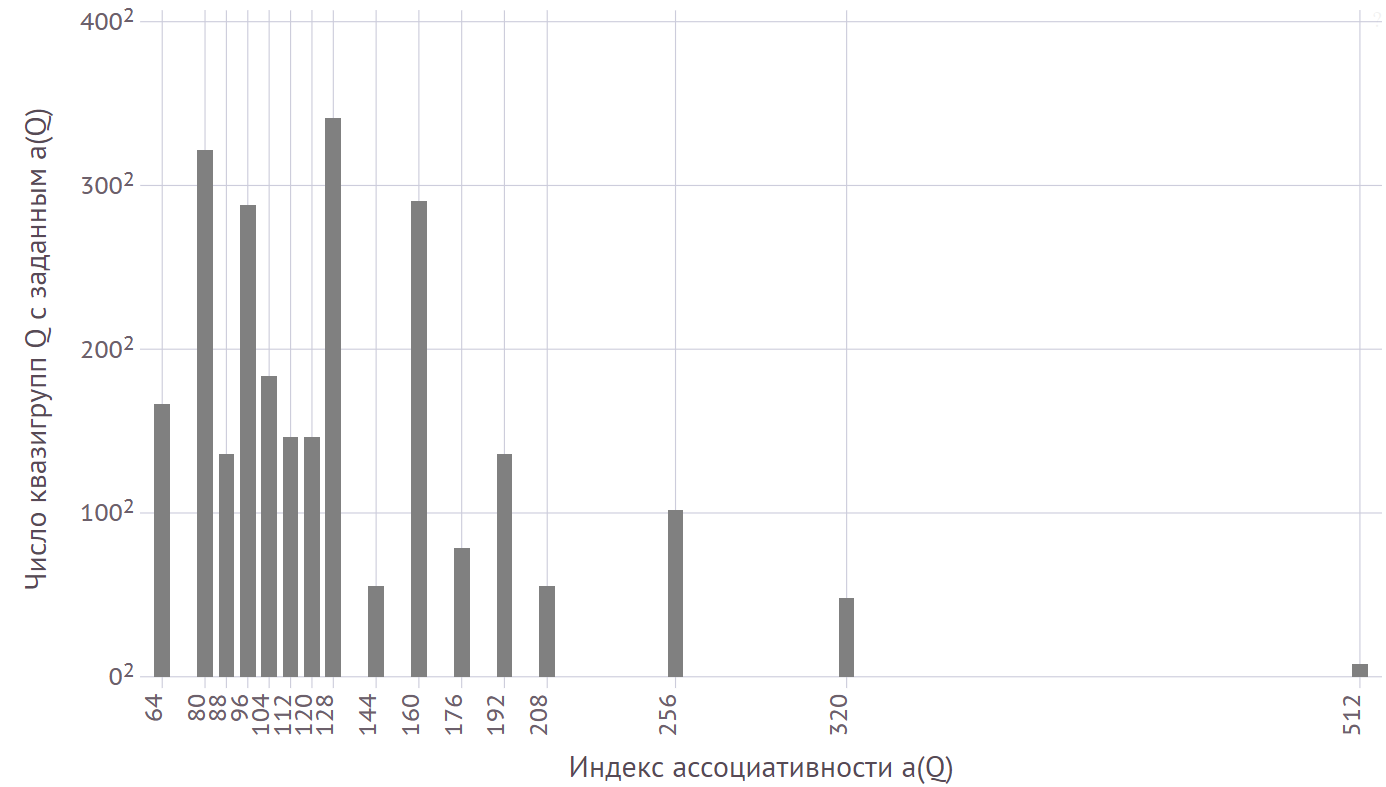
\includegraphics[scale = 0.38]{histogram.png}
            \end{figure}
        \end{column}%
        \hfill%
        \begin{column}{.49\textwidth}
            \begin{figure}[h]
                \centering 
                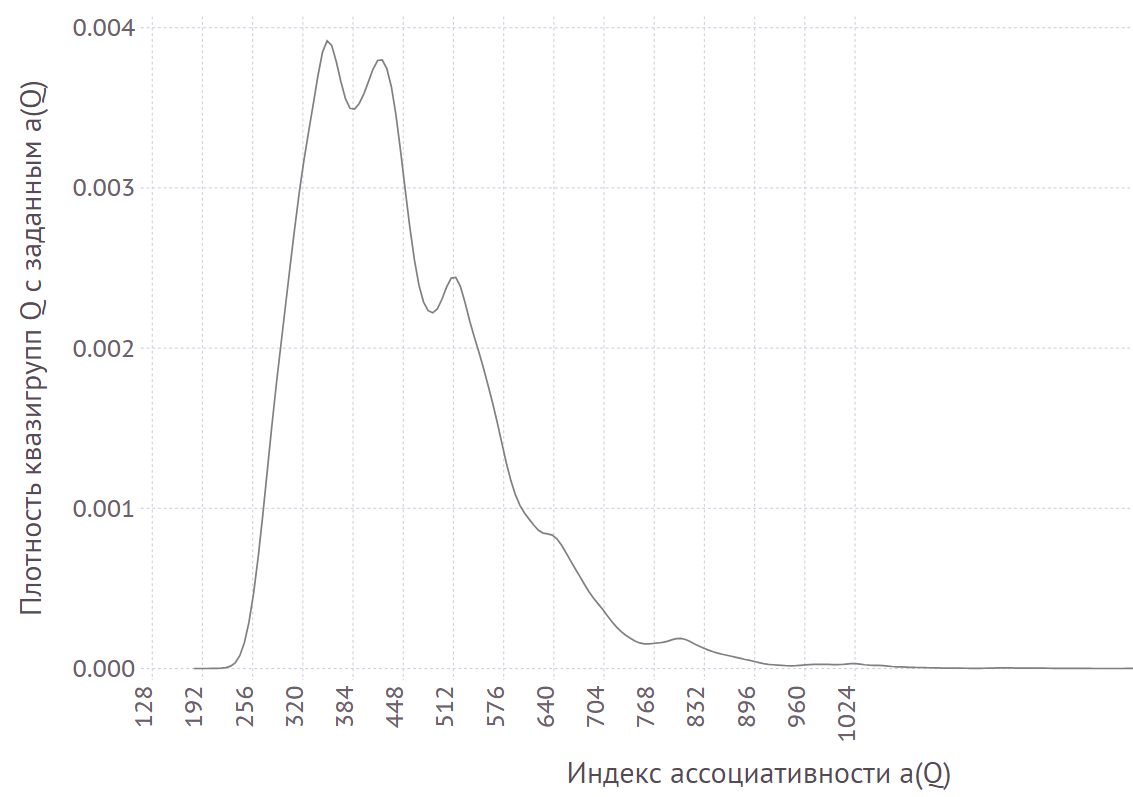
\includegraphics[scale = 0.38]{density.png}
            \end{figure}
        \end{column}%
    \end{columns}  
\end{frame}


\begin{frame}{Подстановки, порождаемые правильными семействами}
    Пусть $\ff \colon Q^n \to Q^n$~--- правильное, $(Q, \circ)$~--- квазигруппа.
    Тогда отображение
    \[ 
        \sigma_\ff(x) \colon x \to x \circ \ff(x),
        \quad
        \begin{bmatrix}
            x_1 \\
            \vdots \\
            x_n
        \end{bmatrix} 
        \to 
        \begin{bmatrix}
            x_1 \circ f_1(x_1, \ldots, x_n) \\
            \vdots \\
            x_n \circ f_n(x_1, \ldots, x_n)
        \end{bmatrix}
    \]
    является подстановкой: $\sigma_{\ff} \in Perm(Q^n)$.
\end{frame}


\begin{frame}
    Пусть $\ff \colon Q^n \to Q^n$~--- правильное.
    Рассмотрим $\sigma^{-1}_{\ff} \in Perm(Q^n)$.
    \begin{mytheorem}{Обратимость \textquote{правильных подстановок}}
        Если $(Q, +)$~--- группа (т.е., операция $+$ ассоциативна), то семейство $\gf \colon Q^n \to Q^n$, определенное равенством
        \[
            \gf(x) = (-x) + \sigma_{\ff}^{-1}(x)
        \]
        также является правильным.
    \end{mytheorem}
    \pause
    Т.е., если $\ff$~--- правильное, то существует правильное семейство $\gf$ со свойством
    \[
        \sigma^{-1}_{\ff}(x) = \sigma_{\gf}(x).
    \]
    \pause
    Таким образом, множество \textquote{правильных подстановок} замкнуто относительно взятия обратного элемента (в случае, когда $Q$~--- группа).
\end{frame}


\begin{frame}{О подстановках, порождаемых правильными семействами-2}
    Множество \textquote{правильных подстановок}$\sprop$ \textbf{не является} подгруппой $Perm(Q^n)$.
    
    \pause 
    \begin{mytheorem}{Транзитивность действия}
        Замыкание $\sprop$ действует транзитивно на $Q^n$ (любой элемент из $Q^n$ можно перевести в любой другой с помощью композиции некоторого количества $\sigma_{F}$).
    \end{mytheorem}
    \pause 
    \begin{mypropos}{Булев случай}
        При $Q = \EE_2$ замыкание $\sigma_{\ff}$ порождает все множество подстановок $Perm(\EE_2^n)$.
        \footcitetext{USOphd}
    \end{mypropos}
\end{frame}


\begin{frame}{О подстановках, порождаемых правильными семействами-3}
    Пусть $\ff$~--- правильное семейство булевых функций.
    \begin{mytheorem}{Четность числа элементов в прообразе}
    \label{thm:preimage}
        Для любого $\alpha \in \{0, 1\}^n$ число решений уравнения $\ff(x) = \alpha$ всегда четно.
    \end{mytheorem}
    \pause
    \begin{mytheorem}{Количество неподвижных точек $\sigma_{\ff}$}
        У подстановки $\sigma_{\ff}(x) = x \oplus {\ff}(x)$ чётное число неподвижных точек.
    \end{mytheorem}
\end{frame}


\begin{frame}{Простота и неаффинность, $n=2$}
    \[
        \xx, \yy \in \ZZ_2^n \quad \xx \circ \yy = \xx \oplus \ff(\xx) \oplus \yy \oplus \gf(\yy).
    \]

    \begin{center}
        \begin{tabular}{|>{\columncolor{Gray}}c|c|c|}
            \hline
            \rowcolor{Gray}
            Свойства & Афинная & Неаффинная \\
            \hline
            Не простая & 112 & 0 \\
            \hline
            Простая & 32 & \textbf{0} \\
            \hline
        \end{tabular}
    \end{center}
\end{frame}


\begin{frame}{Простота и неаффинность, $n=3$}
    \[
        \xx, \yy \in \ZZ_2^n \quad \xx \circ \yy = \xx \oplus \ff(\xx) \oplus \yy \oplus \gf(\yy).
    \]

    \begin{center}
        \begin{tabular}{|>{\columncolor{Gray}}c|c|c|}
            \hline
            \rowcolor{Gray}
            Свойства & Афинная & Неаффинная \\
            \hline
            Не простая & 30784 & 231936 \\
            \hline
            Простая & 9216 & \textbf{281600} \\
            \hline
        \end{tabular}
    \end{center}
\end{frame}


\begin{frame}{Резюме}
    \begin{coloritemize}
        \item Рассмотрены некоторые релевантные с точки зрения криптографии свойства квазигрупп, порождаемых правильными семействами.
        \pause 
        \item Доказан ряд утверждений про индекс ассоциативности получаемых квазигрупп, проведен вычислительный эксперимент для $n = 2, 3, 4$.
        \pause 
        \item Доказан ряд утверждений про подстановки, порождаемые правильными семействами функций; проведен вычислительный эксперимент для проверки простоты и неаффинности для $n = 2, 3$.
    \end{coloritemize}
\end{frame}


\begin{frame}
    \begin{center}
        {\Huge Спасибо за внимание!}
    \end{center}
\end{frame}


% %%% BIBLIOGRAPHY
\begin{frame}[allowframebreaks]{Список литературы}
    \printbibliography
\end{frame}


\end{document}

